% Nyolcadik előadás

\chapter{A vezérlőegység}

A vezérlőegység az egyik legbonyolultabb áramkör a processzoron belül, a felépítése általában titkos.
Célja a vezérlőjelek előállítása.

\section{Fejlődése}
A vezérlőegységeknek két típusa létezik: szekvenciális (centralizált) és párhuzamos (decentralizált).
A párhuzamos vezérlés komplexebb, mint a szekvenciális.
Az első számítógépeknél huzalozott, szekvenciális vezérlést alkalmaztak.

1957-ben változtattak rajta először a mikroprogramozott vezérlés megjelenésével.
1964-ben jelent meg a szuperskalár elv, majd 1967-ben a futószalag.
Ezek a vezérlési módok már komplexitás szerint párhuzamosak voltak, tartalmaztak huzalozott és mikroprogramozott részeket is.

\section{Ütemező}
A vezérlő lelke az ütemező, a szekvenciális vezérlők a vezérlő jelek fix szekvenciáját állítja elő (huzalozott vezérlés).
A párhuzamos elvet követő ütemezők mikroprogramok segítségével állítják elő a vezérlő jeleket.

\section{Huzalozott vezérlő}
\subsection{A tevezés lépései}
\begin{enumerate}
    \item igazságtábla felírása
    \item logikai függvények felírása
    \item azonos átalakítások (egyszerűsítés)
    \item áramköri elemek számának minimalizálása
    \item végrehajtási idő minimalizálása
    \item megvalósítás
\end{enumerate}

\subsection{Előnye}
Mivel előre elkészített áramkörökkel működik programok helyett, nagyon gyors.

\subsection{Hátránya}
A bonyolult áramkör nehezen átlátható, módosítása pedig nehézkes.

\subsection{Működése}
A vezérlés alapvető elve, hogy egy (forrás) regiszter tartalmát egy módosító áramkörön keresztül egy másik (cél) regiszterbe vezetjük.
Műdödési sémája:
\begin{figure}[H]
    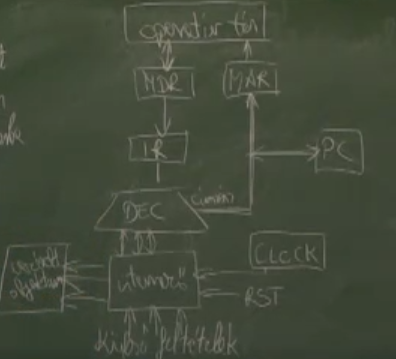
\includegraphics[width=0.8\textwidth]{vez}
    \centering
    \caption{A huzalozott vezérlő működési elve}
    \label{fig:vez}
\end{figure}
Az ütemező feladata az összes többi objektum vezérlése.
Ilyen objektumok pl.:
\begin{itemize}
    \item buszok
    \item ALU
    \item PC
    \item IR
    \item IO
    \item adatutak
\end{itemize}
A módosító áramkörök léptethetik, invertálhatják, komparálhatják az adatokat.
A vezérlő feladata még a kapuáramkörök megnyitása is. 

\section{Mikroprogramozott vezérlő}
A huzalozotthoz képest átláthatóbb, könnyen módosítható, viszont lassú.
A vezérlőjeleket egy mikroprogram állítja elő.
Minden CPU utasítás egy vagy több mikroutasítással valósul meg.
A mikroművelet aktivál egy specifikus vezérlő vonalkészletet.
A mikroprogram kimenete a vezérlő jel.
A mikroprogram fejlesztése nagy hardverismeretet igényel, ezért a gyártók írják a saját processzoraikhoz.

A mai processzorok kombinálják a huzalozott és a mikroprogramozott vezérlést.